\chapter{Trave: progetto e verifica agli SLU per taglio}\label{chap:traveTaglio}
Una volta concluso il progetto e la verifica delle armature longitudinali per effetto dell'azione flessionale, si passa al dimensionamento dell'armatura trasversale. Bisogna comunque assicurarsi che la sezione in calcestruzzo sia in grado di sopportare gli sforzi generati dall'azione tagliante e, in caso contrario, è necessario riprogettarla. 

Il diagramma di inviluppo del taglio sulla trave è stato riportato precedentemente in figura~\ref{fig:shearEnvelope_slu} a pagina~\pageref{fig:shearEnvelope_slu}, mentre i valori sugli appoggi sono presenti nella tabella~\ref{tab:shear_slu} di pagina~\pageref{tab:shear_slu}.

Seguendo quando descritto nelle \ntc al capitolo \textbf{4.1.2.3.5 Resistenza nei confronti di sollecitazioni taglianti}, anche se non necessaria si deve disporre un'armatura trasversale minima (di staffe)
\[
A_{st,min} = 1.5\,b\,\left[\dfrac{mm^2}{m}\right] = 1.5\cdot 300 = 450\,\dfrac{mm^2}{m}
\]
e comunque non minore di \emph{tre staffe al metro}. Il passo massimo delle staffe deve essere di
\[
s_{max} = \min\left\{0.8\,d; \dfrac{1000\,mm}{3}; 15\Phi_l\right\} =\min\left\{368\,mm; 333.33\,mm; 270\,mm\right\} = 270\,mm
\]

Il calcolo della quantità di staffe da disporre nella trave è preceduto dalla valutazione della resistenza a taglio della trava senza armatura trasversale; se
\[
V_{Rd} \geq V_{Ed}
\]
è sufficiente l'armatura minima secondo quanto scritto poco sopra. In caso contrario si passa al calcolo esplicito delle staffe.

Per comidità i valori del taglio sollecitante ai nodi sono raggruppati e ordinati nel seguente vettore (in valore assoluto)
\[
\underline{V_{Ed}} = \begin{Bmatrix}
	V_{N1}^{dx} \\  V_{N2}^{sx} \\  V_{N2}^{dx} \\  V_{N3}^{sx} \\  V_{N3}^{dx} \\V_{N4}^{sx} \\  V_{N4}^{dx} \\V_{N5}^{sx} \\  V_{N5}^{dx} \\V_{N6}^{sx} \\  V_{N6}^{dx} \\V_{N7}^{sx}
\end{Bmatrix}
= 
\begin{Bmatrix}
	150.59 \\  245.457 \\  286.437 \\  286.33 \\  272.636 \\  266.498 \\  266.79 \\  261.915 \\  246.693 \\  202.222 \\  208.848 \\  105.286
\end{Bmatrix}\,kN
\]

Il taglio resistente per una trave fessurata senza armatura trasversale è dato dall'effetto pettine e, secondo le \ntc vale
\[
V_{Rd} = \max\left\{\left[\dfrac{0.18\,k\,\left(100\,\rho_1\,f_{ck}\right)^{1/3}}{\gamma_c} + 0.15\,\sigma_{cp}\right]\,b_w\,d; (\nu_{min} + 0.15\,\sigma_{cp})\,b_w\,d\right\}
\]
dove il primo termine deriva dall'effetto pettine, mentre il secondo è conseguenza di prove sperimentali. In particolare
\begin{align*}
	k &= 1+\left(\dfrac{200}{d}\right)^{1/2} \leq 2\\
	\nu_{min} &= 0.035\,k^{3/2}\,f_{ck}^{1/2}\\
	\rho_1 &= \dfrac{A_{sl}}{b_w\,d} \leq 0.02\\
	\sigma_{cp} &= \dfrac{N_{Ed}}{A_c}
\end{align*}
dove $A_{sl}$ è l'area di armatura tesa calcolata nel capitolo~\ref{chap:flessioneTrave_slu}. Essendo $d = 460\,mm$ costante lungo tutto lo sviluppo della trave, $k$ è uguale per tutte le sezioni e vale 
\[k = 1.66 < 2\]
Ne consegue che anche $\nu_{min}$ è costante e vale 
\[
\nu_{min} = 0.3743\,MPa^{1/2}
\]

I valori di $\rho_1$ sono 
\[
\underline{\rho_1} = 
\begin{Bmatrix}
	0.00553193489001681\\
	0.00921989148336135\\
	0.00737591318668908\\
	0.0110638697800336\\
	0.00737591318668908\\
	0.0110638697800336\\
	0.00737591318668908\\
	0.0110638697800336\\
	0.00737591318668908\\
	0.00921989148336135\\
	0.00553193489001681
\end{Bmatrix}
\]

Infine, $b_w = b =300\,mm$, $\gamma_c = 1.5$ e $\sigma_{cp} = 0$. La resistenza a taglio della sezione non armata vale
\[
\underline{V_{Rd}} = 
\begin{Bmatrix}
	65.95969881495\\
	78.2038703603589\\
	72.5980422819886\\
	83.1040129816814\\
	72.5980422819886\\
	83.1040129816814\\
	72.5980422819886\\
	83.1040129816814\\
	72.5980422819886\\
	78.2038703603589\\
	65.95969881495
\end{Bmatrix}\,kN
\]
che è nettamente minore del taglio sollecitante. \textbf{La trave necessita di un'armatura specifica a taglio}, poiché
\[
V_{Rd} \ngeqslant V_{Ed}
\]

\section{Calcolo dell'armatura a taglio}\label{sec:armaturaTaglio}
Il dimensionamento dell'armatura resistente a taglio viene eseguito seguento quanto riportato al punto \textbf{4.1.2.3.5.2} delle \ntc e considerando l'armatura trasversale composta da staffe ($\alpha = 90^\circ$). La resistenza a taglio della sezione è pari al minimo valore tra il taglio trazione sulle armature trasversali e il taglio compressione sui puntoni in calcestruzzo inclinati
\[
V_{Rd} = \min\left\{V_{Rsd}; V_{Rcd}\right\}
\]
dove, nell'ipotesi di staffe ($\alpha = 90$, $\cot\alpha = 0$, $\sin\alpha =1$)
\[
V_{Rsd} = 0.9\,d\,\dfrac{A_{sw}}{s}\,f_{yd}\,\left(\cot\alpha + \cot\theta\right)\,\sin\alpha = 0.9\,d\,\dfrac{A_{sw}}{s}\,f_{yd}\,\cot\theta
\]
e 
\[
V_{Rcd} = 0.9\,d\,b_w\,\alpha_c\,\nu\,f_{cd}\,\dfrac{\cot\alpha + \cot\theta}{1+\cot^2\theta} = 0.9\,d\,b_w\,\alpha_c\,\nu\,f_{cd}\,\dfrac{\cot\theta}{1+\cot^2\theta}
\]

\subsection{Resistenza a taglio massima lato calcestruzzo}

Prima di procedere si deve calcolare la resistenza a taglio massima lato calcestruzzo, che deve essere maggiore del taglio sollecitante. Se così non fosse, sarebbe necessario riprogettare la sezione o tuttalpiù aumentare la classe del calcestruzzo. Il taglio compressione massimo si ha per $\cot\theta = 1$, cioè per $\theta = \frac{\pi}{4}$
\[
V_{Rcd,max} = V_{Rcd}\,(\cot\theta=1) = 439.875\,kN > \max\left\{\underline{V_{Ed}}\right\} = 286.437\,kN
\]
Si deduce che la sezione in calcestruzzo riesce a sopportare il taglio sollecitante.

\subsection{Armatura a taglio in campata}

Si scelgono barre di diametro $8\,mm$ ed essendo delle staffe il numero di bracci è pari a $2$; l'area di una staffa è perciò di
\[
A_{st} = 2\cdot\dfrac{\pi\,8^2}{4} = 32\,\pi\,mm^2 = 100.53\,mm^2
\]

Sono necessarie 
\[
n_{st} = \dfrac{A_{st,min}}{A_{st}} = \dfrac{450\,\frac{mm^2}{m}}{100.53\,mm^2} = 4.476\simeq 5 \dfrac{staffe}{metro}
\]
con un passo di 
\[
s = \dfrac{1000\,mm}{n_{st}} = \dfrac{1000\,mm}{4.476} = 223.41\,mm \simeq 220\,mm < s_{max} = 270\,mm
\]

Questa armatura verrà disposta nella parte centrale delle campate, dove non è necessaria un'armatura specifica a taglio. 

Supponendo una condizione di rottura, cioè per $V_{Rcd} = V_{Rsd}$ con l'armatura appena calcolata e risolvendo in $\theta$, si ottiene l'angolo di inclinazione del puntone di calcestruzzo, pari a
\[
\theta = 0.29431\si{1}  =  \ang{16.86} < \theta_{min} = \ang{21.8}
\]

Si deve fissare $\theta = \theta_{min} = \ang{21.8}$ e sostituendo si calcolano il taglio trazione e il taglio compressione
\begin{align*}
	V_{Rsd}(\theta = \ang{21.8}) &= 185.07\,kN\\
	V_{Rcd}(\theta = \ang{21.8}) &= 303.38\,kN
\end{align*}
il taglio resistente nelle parti centrali delle campate vale
\[
V_{Rd} = \min\{V_{Rsd}; V_{Rcd}\} = V_{Rsd} = 185.07\,kN
\]

\subsection{Armatura a taglio sugli appoggi}
Sugli appoggi è necessario progettare un'armatura specifica che dipende dal valore del taglio sollecitante. Si intuisce che, a parita di diametro delle staffe, l'armatura dovrà essere infittita. Considerando la condizione limite tale per cui $V_{Rcd} = V_{Ed}$ si può calcolare il valore dell'inclinazione $\theta$ dei puntoni in calcestruzzo. Si ottengono i seguenti valori, raggruppati per comodità in un vettore
\[
\theta_{Ed}^{(0)} = \begin{Bmatrix}
	0.17470699017709382\\
	0.2959961165631609\\
	0.35456791598081494\\
	0.3544076777989241\\
	0.3342460477177851\\
	0.325416534901305\\
	0.32583386351374477\\
	0.3189007052015158\\
	0.29769110152969963\\
	0.2388433511793755\\
	0.2473623789331834\\
	0.12085041471779118
\end{Bmatrix} =
\begin{Bmatrix}
	\ang{10.01}\\
	\ang{16.96}\\
	\ang{20.32}\\
	\ang{20.31}\\
	\ang{19.15}\\
	\ang{18.65}\\
	\ang{18.67}\\
	\ang{18.27}\\
	\ang{17.06}\\
	\ang{13.68}\\
	\ang{14.17}\\
	\ang{6.92}
\end{Bmatrix} < \theta_{min} = \ang{21.8}
\]
Si fissano tutti i valori di $\theta$ pari a $\ang{21.8}$. Con questo valore si può calcolare il passo effettivo delle staffe sugli appoggi, assumendo la condizione limite per cui $V_{Rsd} = V_{Ed}$
\[
s_{Ed}^{(0)} = 
\begin{Bmatrix}
	270\\
	160\\
	140\\
	140\\
	140\\
	150\\
	150\\
	150\\
	160\\
	200\\
	190\\
	380
\end{Bmatrix}\,mm~\Longrightarrow~s_{Ed} = 
\begin{Bmatrix}
	220\\
	160\\
	140\\
	140\\
	140\\
	150\\
	150\\
	150\\
	160\\
	200\\
	190\\
	220
\end{Bmatrix}\,mm
\]
dove si è deciso di fissare i valori maggiori della spaziatura massima al valore di spaziatura di campata $s = 220\,mm$

\section{Verifica}
La verifica va fatta in condizioni di collasso, perciò con
\[
V_{Rsd} = V_{Rcd}
\]

Risolvendo si possono calcolare gli angoli $\theta$ effettivamente originati con i valori di passo appena trovati
\[
\theta_{Ed} = 
\begin{Bmatrix}
	\ang{16.86}\\
	\ang{19.89}\\
	\ang{21.32}\\
	\ang{21.32}\\
	\ang{21.32}\\
	\ang{20.57}\\
	\ang{20.57}\\
	\ang{20.57}\\
	\ang{19.89}\\
	\ang{17.71}\\
	\ang{18.19}\\
	\ang{16.86}\\
\end{Bmatrix}~\Longrightarrow~\theta_{Ed} = 
\begin{Bmatrix}
	\ang{21.8}\\
	\ang{21.8}\\
	\ang{21.8}\\
	\ang{21.8}\\
	\ang{21.8}\\
	\ang{21.8}\\
	\ang{21.8}\\
	\ang{21.8}\\
	\ang{21.8}\\
	\ang{21.8}\\
	\ang{21.8}\\
	\ang{21.8}\\
\end{Bmatrix}
\]
e quindi i valori di taglio trazione e di taglio compressione sono
\[
V_{Rsd} = 
\begin{Bmatrix}
	185.08\\
	254.484\\
	290.839\\
	290.839\\
	290.839\\
	271.449\\
	271.449\\
	271.449\\
	254.484\\
	203.587\\
	214.303\\
	185.08
\end{Bmatrix}\,kN\qquad
V_{Rcd} = 
\begin{Bmatrix}
	438.667\\
	438.667\\
	438.667\\
	438.667\\
	438.667\\
	438.667\\
	438.667\\
	438.667\\
	438.667\\
	438.667\\
	438.667\\
	438.667
\end{Bmatrix}\,kN
\]

Il taglio resistente è quello lato acciaio, cioè
\[
V_{Rd} = \begin{Bmatrix}
	150.805\\
	254.484\\
	290.839\\
	290.839\\
	290.839\\
	271.449\\
	271.449\\
	271.449\\
	254.484\\
	203.587\\
	214.303\\
	150.805
\end{Bmatrix}\,kN > V_{Ed} = 
\begin{Bmatrix}
	150.59 \\  245.457 \\  286.437 \\  286.33 \\  272.636 \\  266.498 \\  266.79 \\  261.915 \\  246.693 \\  202.222 \\  208.848 \\  105.286
\end{Bmatrix}\,kN
\]

\begin{figure}
    \centering
	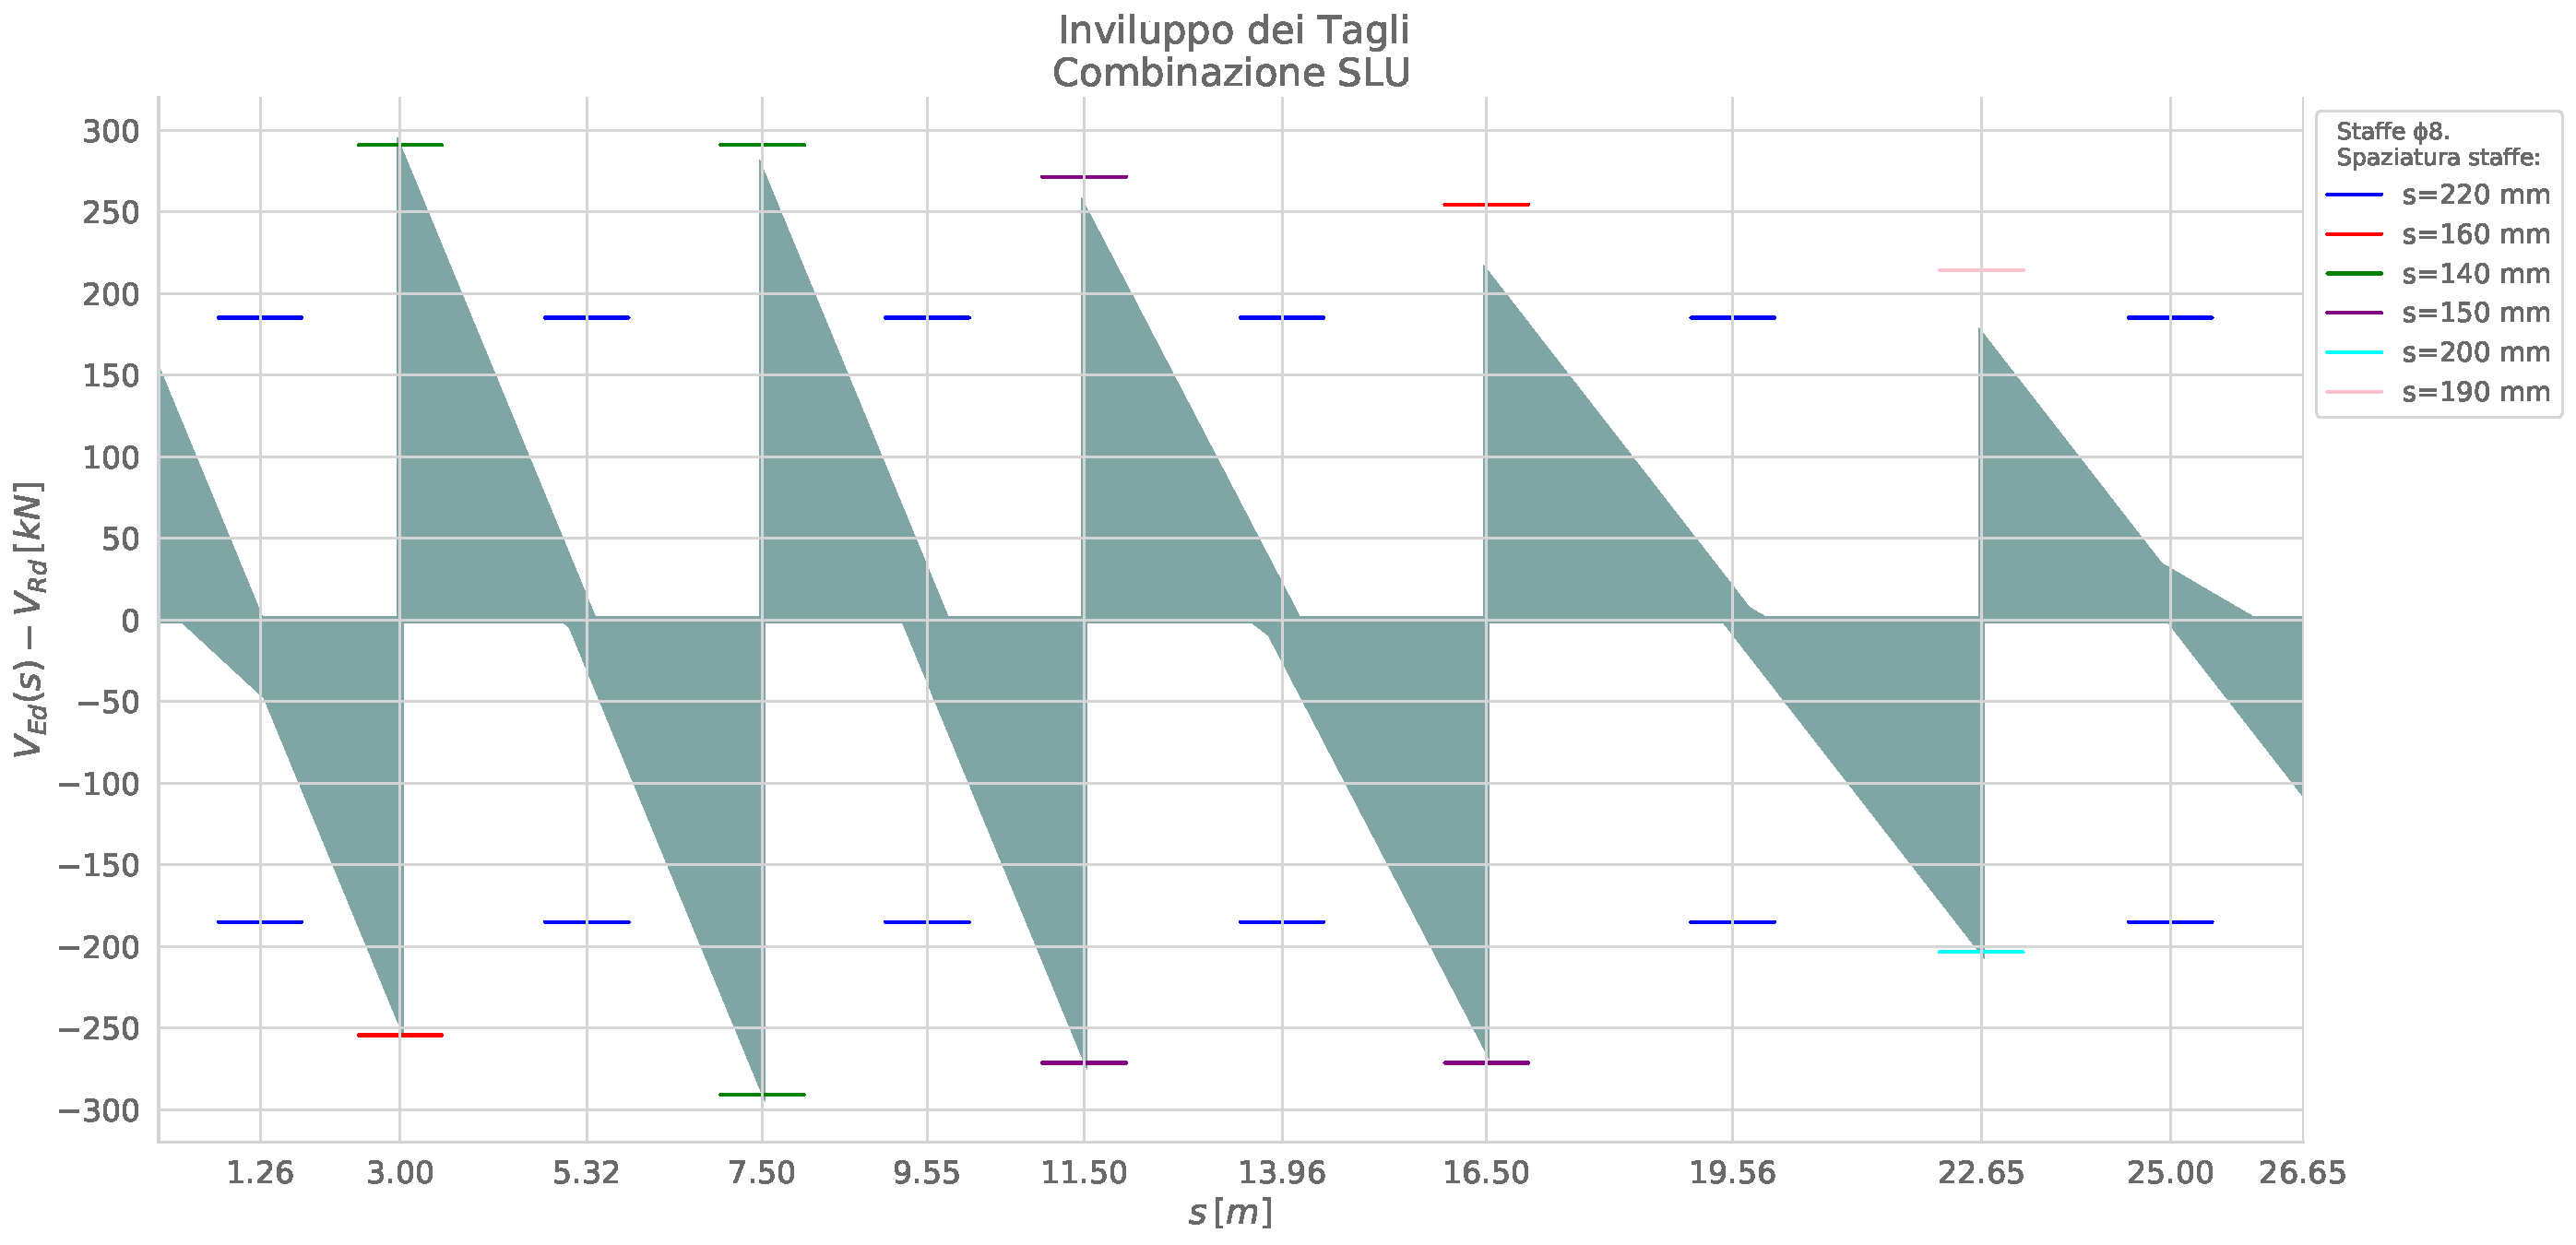
\includegraphics[width=\textwidth]{VEd-VRd}
	\caption{Sovrapposizione taglio sollecitante e taglio resistente}
	\label{fig:VEd-VRd}
\end{figure}
\cleardoublepage
\pagebreak
\thispagestyle{empty}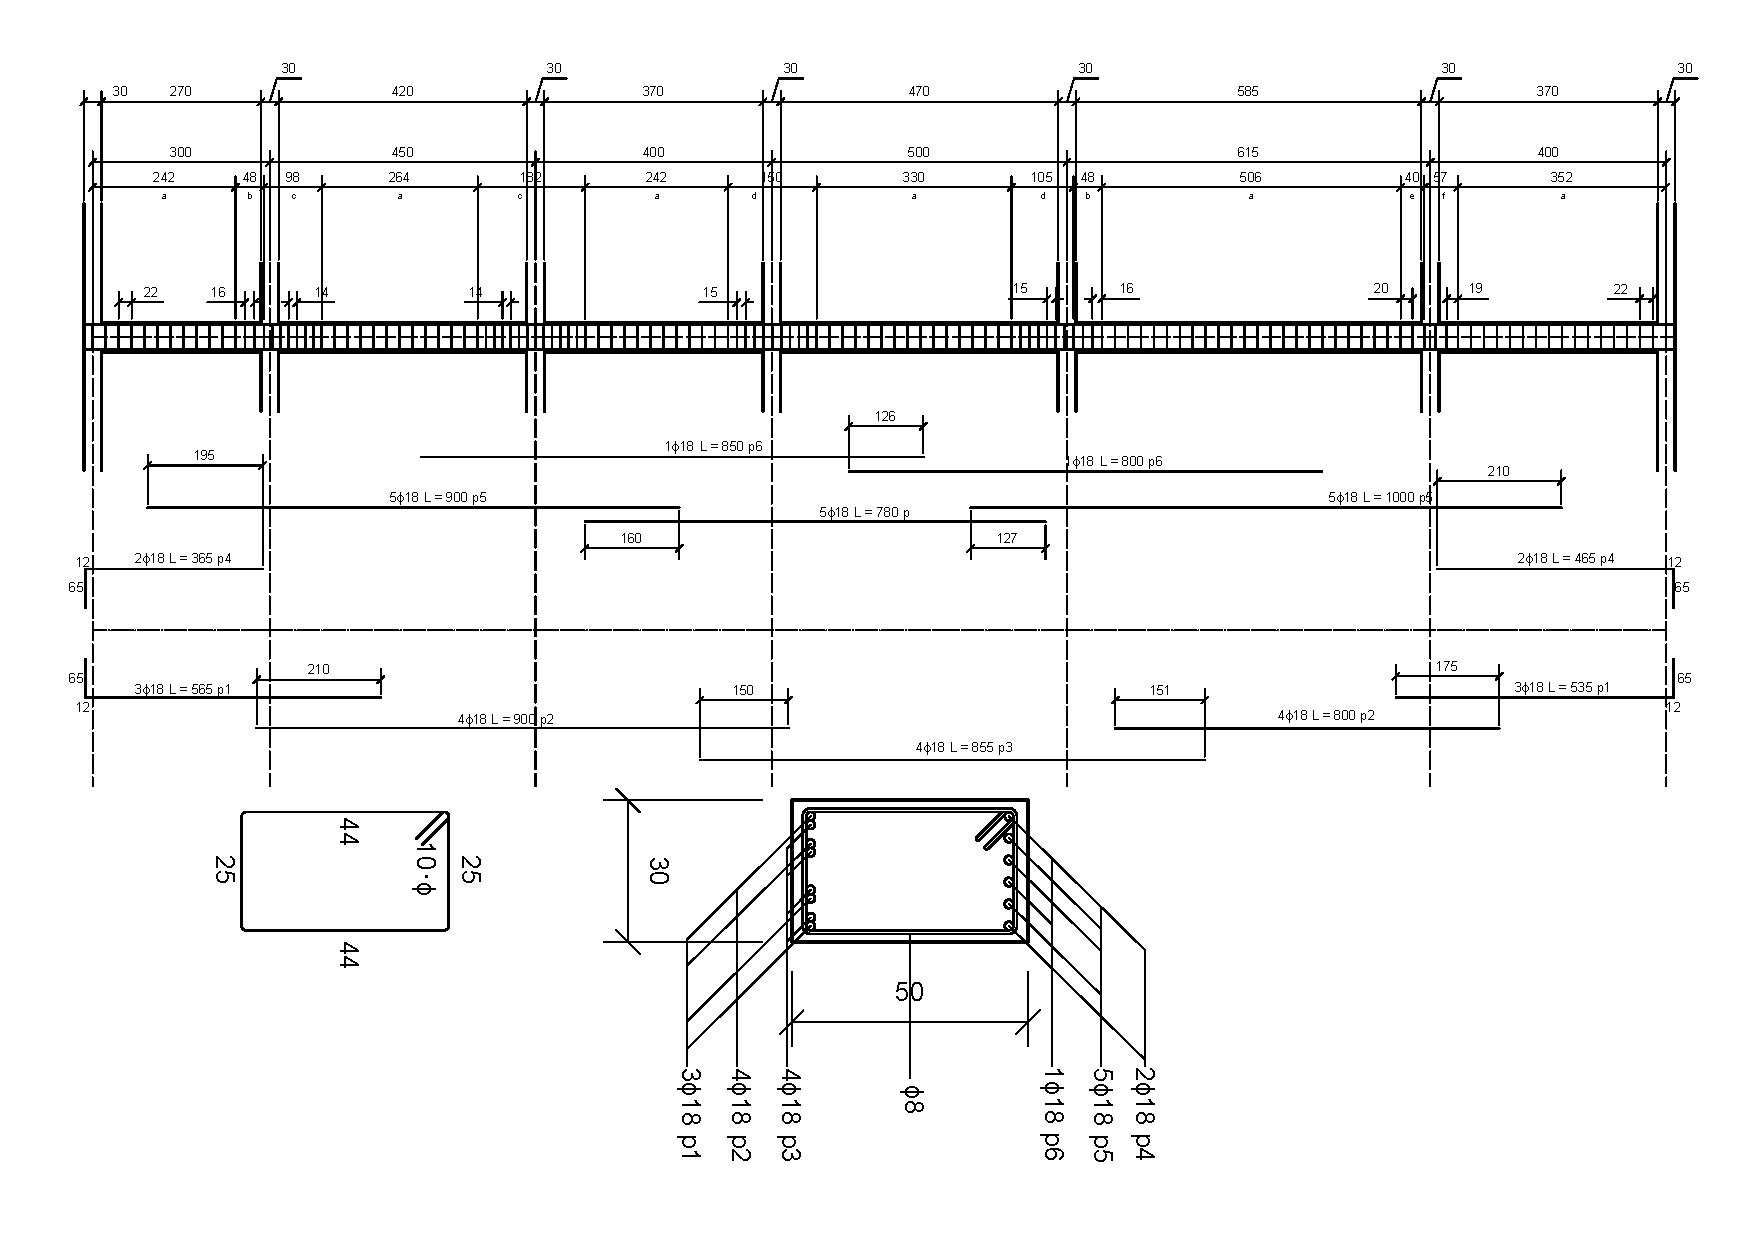
\includepdf[pages=1,pagecommand={}, angle=90, width=\textwidth]{../../disposizioneArmatureTaglio}
\cleardoublepage
